
%
%  $Description: Author guidelines and sample document in LaTeX 2.09$ 
%
%  $Author: ienne $
%  $Date: 1995/09/15 15:20:59 $
%  $Revision: 1.4 $
%

\documentclass[times, 10pt,twocolumn]{article} 
\usepackage{latex8}
\usepackage{times}

\usepackage{graphicx} %sjr added
\graphicspath{{../presentation/figures/}{../draft/figures/}}
%\documentstyle[times,art10,twocolumn,latex8]{article}

%------------------------------------------------------------------------- 
% take the % away on next line to produce the final camera-ready version 
\pagestyle{empty}

%------------------------------------------------------------------------- 
\begin{document}

\title{Effects of Irregular Topology in Spherical Self-Organizing Maps}

\author{
Charles R. Schmidt\\
School of Geographical Sciences\\Arizona State University\\
Charles.R.Schmidt@asu.edu\and
Sergio J. Rey\\
School of Geographical Sciences\\Arizona State University\\srey@asu.edu
\and
Andr\'e Skupin\\
Department of Geography\\San Diego State University\\
skupin@mail.sdsu.edu
}

\maketitle
\thispagestyle{empty}

\begin{abstract}
We explore the effect of different topologies on properties of self-organizing
maps (SOM). We suggest several diagnostics for measuring
topology-induced errors in SOM and use these in a comparison of four different
topologies. The results $\ldots$
  
\end{abstract}



%------------------------------------------------------------------------- 
\Section{Introduction}

The Self-Organizing Map (SOM) is an unsupervised competitive learning process
developed by Teuvo Kohonen as a technique to analyze and visualize high
dimensional data sets.  The applications of SOM are far reaching;
Kohonen \cite{Kohonen2000} provides a thorough review of the SOM literature including
applications of SOM.  SOM has been used in applications ranging from speech
recognition and image classification to breast cancer detection and gene
expression clustering.  Agarwal
and Skupin \cite{skupin07} outline the growing interest of SOM to
the GISciences, and propose that the relationship between SOM and GIScience
should be bidirectional.  The SOM offers a powerful method for exploring and
visualizing geographic data and GIScience offers a wide array of tools
and methods to enable the exploration of the SOM itself.  The exploration of
spatial relationships has always been of great interest to geographers, and as
Ritter
\cite{ritter99} states, the goal of SOM is ``to translate \emph{data
similarities} into \emph{spatial relationships}'' \cite[p. 1]{ritter99}. 

The SOM is a type of artificial neural network in which neurons are ``organized''
in such a way as to project the high-dimensional relationships of a set of
training data onto a low-dimensional network structure.  The traditional
SOM uses a rectangular or hexagonal network topology \cite{Kohonen2000}.  These topologies 
create a well-known problem in SOM called the boundary or edge effect.  Neurons on
the boundary of the hexagonal and rectangular lattices have fewer neighbors,
which reduces their ability to interact with other neurons during the
self-organizing process.  Using a spherical lattice has been widely suggested as a
solution to the problem \cite{ritter99, boudjemai2003, sangole03,
Nishio:2006fk, wu2006}. The use of the spherical lattice, however, does not
completely overcome the boundary problem, and the choice of which spherical
topology to use for the network can be difficult to make.

A regular network topology is one in which every node on the network has exactly the
same number of adjacent nodes.  Any topology involving an edge is irregular.
Arranging our lattice on the surface of a sphere seems to be an obvious
way to overcome the edge.  However, there exist only five arrangements on the
sphere which are completely regular; these are the five platonic solids \cite{ritter99,
harris2000}.  Any other arrangement of neurons on the surface of the sphere will
result in an irregular topology, as not all neurons will have the same number of
neighbors.

The classic method for minimizing this irregularity is to generate
the spherical lattice by tessellating (subdividing) the sides of the icosahedron
\cite{Nishio:2006fk}.  While this method will always result in a highly
regular spherical topology, the main drawback is that the number of neurons in
the network (the network size), \(N\), grows exponentially as tessellations are
applied. That results in only very coarse control over network size.
 Other methods for arranging neurons on the sphere allow
for unlimited control over network size, but yield topologies with increased
irregularity \cite{harris2000, wu2005, Nishio:2006fk}.  To date the
literature has largely ignored the more irregular methods in favor of the
aforementioned tessellation-based methods.  A topology which yields a more flexible network
size may be desirable.  However, in order to address this issue of network
size, we must first determine the degree to which irregularity effects the
SOM.

\Section{Edge Effects}

An intrinsic problem with SOMs in two dimensions is the so called edge
effect. This is illustrated in  in Figure \ref{f:edge}, which displays a SOM
trained on socioeconomic census data consisting of 32 variables for US states.
The darker a neuron in the figure, the larger is the distance between the
 neuron and mean of the input vectors. The distance between each of the
 original observations (states) and the mean is represented by a graduated
 circle. Taken these two together it is clear that the outlier observations
 are pushed towards the edges of the map, while the observations that are
 closest to the multidimensional center of the data are assigned to central
 neurons on the map.

At the edge of the map, neurons have fewer neighbors which results in any
observations being assigned to them having fewer competitive signals. At the
same time, the edge of the neural lattice represents a true visual boundary
which affects its ability to represent data similarities as spatial
relationships.

\begin{figure}
  \begin{center}
\caption{Edge effects in SOM}\label{f:edge}
  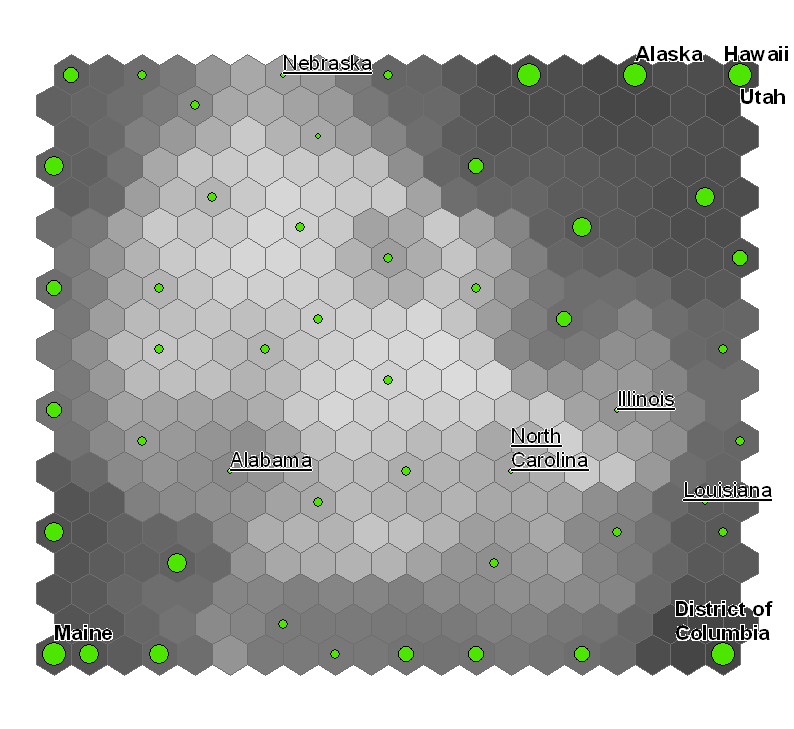
\includegraphics[width=0.70\linewidth]{states.png}
\end{center}
\end{figure}

One way to eliminate the edge effect is to wrap the lattice around a
three-dimensional object such as a sphere or torus, thereby removing the edge
entirely. The toroidal SOM was introduced by \cite{li1993}, however the torus
is not effective for visualization, as maps generated from a torus are not
very intuitive \cite{ito2000,wu2006}.  \cite{ritter99} describes the torus as
being topologically flat and suggests that a curved topology, such as that of
a sphere, may better reflect directional data.  A sphere also results in a
more intuitive map, since we are accustomed to looking at geographic maps
based on a sphere.  

\label{bg:sphere}
Ritter \cite{ritter99} first introduced the spherical SOM, and several enhancements have
since been suggested \cite{boudjemai2003,sangole03,Nishio:2006fk,wu2006}.  A
good comparison of these enhancements can be found in Wu and Takatsuka
 \cite{wu2006}.  All of
these methods derive their spherical structure through the tessellation of a
polyhedron as originally proposed by Ritter \cite{ritter99}.  Wu and Takatsuka \cite{wu2006} point
out the importance of a uniform distribution on the sphere, and that it is
preferable for all neurons to have an equal number of neighbors and to be
equally spaced.  They find generally that the tessellation method best satisfies
these conditions, and specifically that the icosahedron is the best starting
point \cite{wu2005}. Tessellation of the icosahedron results in a network of
neurons, each having exactly six neighbors, save the original twelve
which each have five neighbors.  This is very close to the ideal structure in
which every neuron would have exactly six neighbors.  \cite{wu2006} prefer
these this structure, because it has very low variances in both neuron spacing
and neighborhood size. 

Based solely on measures of neuron spacing, \cite{wu2005} dismissed the usefulness of a method
proposed by \cite{Rakhmanov94} for distributing points on a sphere.  Similarly
\cite{Nishio:2006fk} use these variance measures to support their helix
algorithm for distributing points on a sphere.  However,
these metrics can be misleading and comparison across topologies may not be
consistent.  The traditional rectangular and hexagonal topologies have no
variance in neuron spacing, and the generally preferred hexagonal structure
displays greater variance in neighborhood size than the rectangular structure.
The torus, by comparison, would have variance in neuron spacing, yet no
variance in neighborhood size.  The distance between two neurons is only
considered during the formation of the neural network.  At this stage the
spacing is significant as it plays a part in constructing the network's
topology by determining neuron adjacency.  However, using this measure to
evaluate potential topologies for use in SOM may be misleading.

As spherical (and other alternative) topologies become
increasingly more common it is necessary to investigate how the choice of
topology effects the SOM.  In this thesis the effect of irregularity within
topologies is studied as an attempt to investigate not only the edge effect,
but also to help facilitate the comparison of topologies.  It is important to
note that spherical topologies may not be appropriate for all applications.
Removing the edge may reduce the SOM's ability to converge.  As outliers are
forced to interact they introduce more competition among the neurons.  We
would also expect outliers to occupy more space in the final map as their
dissimilarity in attribute space should translate to more distant spatial
relationships in the trained SOM.  More research will be needed to help researches
determine the most appropriate topology for their data and research objectives.

In this paper we explore the general utility of certain irregular spherical
topologies beyond offering greater control over network size. We develop and
test new diagnostics to measure and visualize topology-induced errors in SOM.
More specifically we examine the



\Section{Methods}
\chapter{METHODOLOGY}
This chapter is composed of four sections.
Section \ref{meth:som} describes PySOM, our own graph based implementation of
SOM. PySOM provides the necessary inputs to our three diagnostics as described
in section \ref{meth:diag}.  These diagnostics were developed to help
understand how irregularities in topology effect the SOM. To use these
diagnostics we must train several SOMs with comparable training data and
parameters.  The specifics of our training data are explained in section
\ref{meth:data}.  Section \ref{meth:train} describes the training parameters used
across all our SOMs.

\section{Graph based implementation of SOM}
\label{meth:som}
The most widely available implementation of SOM is Kohonen's
own SOM\_PAK \citep{kohonen1996}.  SOM\_PAK implements both the traditional
rectangular and hexagonal topologies.  However, implementations of the
geodesic and spherical SOMs were not readily available at the time this thesis
was written.  In order to test these topologies it was necessary to implement
our own version of SOM, PySOM.  Because the goal of this thesis was to study
different topologies for use in SOM, we created PySOM to be topology agnostic.
That is, our implementation is not explicitly aware of the topology.  Rather, we
represent the topology of the SOM as a graph. The graph provides the necessary
information to determine neuron adjacency and construct neighborhoods.  The
nodes in the graph are pointers to the reference vectors ($m_i$).

To allow for rapid development and cross-platform support we choose to write PySOM
in the Python programing language. As noted by \cite{Rey2006} Python is an
object-oriented programing language that is becoming increasingly popular in
scientific computing. PySOM is maintained as an open-source project is hopes
of facilitating collaboration and further research.  In its present form
PySOM has no user interface, however it is written as a Python library which
allows all of its functionality to be accessed programmatically. %spell checked with google

By abstracting the topology, PySOM can train a SOM using any topology for
which a graph structure can be created. We leverage an existing graph library,
NetworkX, to represent our topologies \citep{networkx}.  Our neighborhood
functions are built on top of this library.  Apart from our neighborhood
search functions, our implementation follows the original incremental SOM
algorithm that is described by \cite{Kohonen2000}.  We store our trained SOM
in a similar fashion as SOM\_PAK.  The reference vectors are represented in a
simple text file.  These ``codebook'' files contain a description of the
topology and other training parameters in the first line of the file.  Each
subsequent line lists the values for the parametric reference vectors, $m_i$,
of the SOM's neurons \citep{kohonen1996}. In addition to this codebook file we
also store the graph as a serialized python object.  Creating the graph
structures for the spherical topologies is considerable more complex and
requires more computation than the traditional topologies.

We provide utility functions to create the graph structures for both the
rectangular and hexagonal topologies.  To create the graph structure for the
geodesic topology we use the ``dome'' software package, which outputs the
point coordinates in ``XYZ'' format for each neuron \citep{dome}.  These
coordinates are fed into the STRIPACK software program. STRIPACK computes both
the Voronoi cells and their complement, the Delaunay triangulation, on the
surface of the sphere \citep{Ranka97}.  The Delaunay triangulation provides the graph
structure between the neurons of the geodesic SOM.  A similar process is used
for the spherical topology. In this case we wrote a python implementation of
the method for distributing points on a sphere that was introduced by
\cite{Rakhmanov94}.  Once again the coordinates are fed into STRIPACK.
An additional utility program reads the output from STRIPACK and
creates the NetworkX graph structure.  PySOM has no direct graphical
output, however several utility functions are provided to assist in the
create of visualizations.  These functions create files that are compatible with
popular GIS software packages, namely ESRI's ArcGIS.

\section{Diagnostics}
\label{meth:diag}
In traditional SOMs, outlying observations are pushed to the edge of the map
where they encounter fewer competing signals.  A prime example of this is the
``Utah-Hawaii'' case shown in Figure \ref{som:states}.  Relying only on the
SOM, one would be left to believe that the two states are similar.  Recalling
that the QError measures the distance between two vectors in attribute space,
we see that the QError from Utah to the neuron is $1.509$, the QError from
Hawaii to the neuron in $1.505$, but the QError from Utah to Hawaii is
$3.014$. In this case only Utah and Hawaii were mapped to that neuron.  In a
case where multiple observations land on the same neuron, it is possible to
measure the average pairwise QErrors between those observations.  This gives us a
notion of internal heterogeneity, \(H\), for each neuron.  We define the
internal heterogeneity of neuron \(i\) as,
 \begin{equation}
   {H_i} = \frac{2}{{n_i}^2-{n_i}}\sum_{j=1}^{n_i}\sum_{k=j+1}^{n_i} ||{x_{ij}}-{x_{ik}}||
 \label{eqno1}
 \end{equation}
where, \(n_i\) is the number of observations mapped to \(i\), and \(x_i\) are
the input vectors mapped to \(i\).  For any neuron that captures more then one
observation, this measure tells how dissimilar those observations are.

The edge effects in SOM make it clear that the compression of the input-space is
not uniform through out a trained map.  While outliers being pushed to the edge of
the SOM is not necessarily an undesirable outcome, it is important understand
when and where information is being compressed.  This variable compression of
the input-space is what allows the SOM to represent high-dimensional data, but
it can also mislead the viewer.  Observing the internal heterogeneity of
neurons may shed light on the patterns of compression.  

More specifically we have developed diagnostics that explore how irregularities
in the topology of the SOM effect this internal heterogeneity.  We compare the
internal heterogeneity at the scale of the neuron and the overall map.  Each
diagnostic was designed to answer a specific research question.  The first
diagnostic addresses the research question regarding the internal
heterogeneity and neighborhood size.  The second diagnostic addresses the
question concerning internal heterogeneity and topological irregularity.  The
third helps visualize the patterns between internal heterogeneity; the
usefulness of which is examined in the next chapter.

\subsection{Internal heterogeneity vs. first-order neighborhood size}
\label{q1}
This diagnostic compares the internal heterogeneity of each neuron against
then neuron's first-order neighborhood size.  It would be expected that in
traditional SOMs neurons closer to the edge, those with fewer neighbors, will
have higher internal heterogeneity. Neurons on the edge of the traditional
(rectangular and hexagonal) topologies are considered more irregular, because
they have few neighbors then neurons inside the edge.  This can be extended to
spherical SOMs by considering the degree of any given neuron.  The degree of a
neuron $deg(m_i)$ measures the number of adjacent neurons.  If the
relationship between $H_i$ and $deg(m_i)$ is consistent across topologies,
neurons with lower degrees should display higher internal heterogeneity.

To implement this diagnostic we calculate the internal heterogeneity ($H_i$)
and degree ($deg(m_i)$) of each neuron. The neurons are then separated into a small number of
groups based on the degree.  For most topologies the number of
different degrees will be limited to three or four.  The variance and mean
is calculated for each of these groups.  The expected result is that
variances and means of the groups will decrease as the degree increases.  This
hypothesis is tested using random labeling as described by \cite{siss2004}.
In random labeling, we randomly assign our calculated $H$ values to the
neurons and recompute the mean and variance of the groups.  We do this many times,
9999 in our case, in order to approximate the true distribution. Finally we
calculate pseudo p-values by comparing our observed mean and variance values
with the simulated distributions.  The results are also visualized using
box-and-whisker diagrams. Box-and-whisker diagrams, or box plots, show the
properties of a distribution.  The diagram shows the mean, first and second
standard deviations, and outliers that extend beyond the second deviation.

One problem that we face in this diagnostic is a small sample size when the neurons of a given
SOM are grouped by their degree.  For example, the four corners of the
rectangular topology are the only neurons that have a degree of two.  The rest
of the neurons have three or four neighbors depending on whether or not they
are on the edge. To address the problem of small sample size for topologies
with relatively few neurons of a particular degree, we will increase
the sample size by combining the results of many SOMs.

\subsection{Internal heterogeneity vs. topological regularity}
This diagnostic compares the internal heterogeneity of each neuron against a
measure of regularity for its associated topology.  As mentioned above the
degree of each neuron measures the number of adjacent neighbors.  A completely
regular network topology (i.e. the torus) has no variance between these
measures.  For irregular networks the variance between these degrees gives us
a measure of irregularity. This particular measure is known as degree
centrality.  The degree of a node on a network is a measure of its centrality, or
importance. Nodes with more connections are thought to be more central to the
network and have a larger influence than nodes with fewer connections.

This holds with our understanding of the edge effect.  Neurons on the edge are
less central to the network and have less influence than other nodes.  These
edge nodes are also less influenced by the network, allowing outliers take
root.  During the training process observations that are more average than
others tend to be centralized.  The observations that surround them tend to be
more extreme.  If you refer back to figure \ref{som:states}, you'll notice
that observations with smaller symbols are closer to the mean of the
input-space and that these observations have been centralized in the network.
Using the degree as a measure of centrality does not capture this picture
well, as neurons near the edge can still have a large degree.  A better way to
capture this effect is to look at closeness centrality, which is the
inverse of the average distance of a neuron to every other neuron on the
network.

Closeness centrality provides a more complete measure of connectedness in a
given topology than degree centrality.  In this diagnostic we compare the
internal heterogeneity of the neurons against the average closeness centrality
of their respective topologies.  This results in one group of internal
heterogeneity measurements for each topology tested.  We evaluated this
diagnostic in much the same way as the last.  We compare the variances and
means of each group, testing for differences with random labeling.  It is
expected that the distribution of internal heterogeneity will be narrower for
groups trained on more regular topologies.  It is further hypothesized that
the mean of internal heterogeneity will decrease when the network is more
regular.  In addition to testing these assumptions with random labeling we
visualize the results with box plots.

\subsection{Visualize internal heterogeneity mapping}
Visualizing the internal heterogeneity may yield insight into how irregular topology
effects the SOM.  Creating these visualization for many different topologies
however, offers a number of challenges.  While the rectangular and hexagonal
topologies are rather straight forward to visualize, the spherical and geodesic
topologies are significantly more involved.  In order to leverage the utility
of existing GIS software we represent our topologies in a form that
these software packages understand.  Toward that end we create polygon layers
in which each polygon represents a neuron.  Shared borders represent
connections between neurons.  Creating the polygons for these topologies
required that we first compute the Voronoi diagram on the surface of the
sphere.  This is done using STRIPACK, a software program created by
\cite{Ranka97}.  Despite the prevalence of spherical coordinates
in GIS, modern GIS software packages have their roots in CAD software. As such
they all assume Cartesian distances and thus can not handle polygons that
cross the $180^{th}$ meridian.  To accommodate this we split each polygon at
the $180^{th}$ meridian and redraw it as two parts.

Once the GIS layers have been created and the internal heterogeneity of each
neuron has been calculated, a number visualizations become possible. We
visualize the internal heterogeneity by shading the corresponding polygons.
These visualizations allow for the exploration of patterns in internal
heterogeneity with relation to the underlaying topology.  Further we can
visualize the component planes, which show how the higher dimensions are
represented in the various SOMs.  We also map our synthetic data back onto the SOM in
order to calculate cluster membership of the neurons.  Visualizing cluster
membership clearly shows how the various topologies perform clustering.


\section{Data}
\label{meth:data}
%Comment from Skupin...
%This section is obviously leaving most of the specifics of the synthetic data
%generation out, which is problematic. I'm willing to go along with this for
%the proposal though, unless it gets raised by the third committee member
Our internal heterogeneity measure is sensitive to both the properties of the SOM
and the properties of the training data. Therefore, a dataset with uniform
properties is needed. We follow the method for generating uniform synthetic
data used by \cite{wu2006}.  Their method creates seven clusters in three
dimensions.  Each cluster is normally distributed and has a standard deviation
of one.  The clusters are centered at the origin and ten units out in each
directions on the x, y and z axes. The uniform clusters generated by this method allow us to
systematically compare the diagnostics under several different topologies.  To
ensure that we can calculate an internal heterogeneity for as many neurons as
possible, we create approximately $25,000$ observations in each dataset.  As
described in the next section, our SOMs have either 642 or 644 neurons
(depending on the topology).  Having a large number of observation relative to
the number of neurons will force the SOM to preform clustering, increasing the
number of neurons for which the internal heterogeneity can be computed.

As mentioned in section \ref{q1} we will need to combine the results of
multiple SOMs in order to ensure a large enough sample size.  To accomplish
this we will create ten synthetic datasets as described above.  Each of these
datasets can be thought of as samples from the same input space.  That is, the
data generating process remains the same for each synthetic dataset created.
After training ten SOMs for each topology we take the average internal
heterogeneity of each to ensure that the results are comparable.


%We will create a number of different data sets and use them to train various SOMs.  

%the data is generated in such a way to increase the probability that each neuron will be occupied by more than one observation.

%Initially the synthetic data for this thesis came from a Gaussian cluster
%generator which creates clusters by randomly sampling from multivariate
%normal distributions \citep{handl}.  \citeauthor{handl}' method to keep
%clusters from overlapping is to create one cluster at a time, with each new
%cluster checked to see if it overlaps with an existing cluster. If it does,
%it is rejected.  The generator continues until the desired number of
%non-overlapping clusters has been reached.  This method tends to create
%clusters of very different shapes and sizes (or extents).

%The limit to using this method for creating data became evident when we
%realized that the internal variance measure was being affected by the
%structure of the clusters.  The internal variance essentially looks at the
%portion of a cluster that is mapped to a particular neuron and measures the
%density.  Because we specify that each cluster contain an equal number of
%observations, they tend to get equal representation (in terms of number of
%neurons) on the trained SOM.  The result of all this is that the smaller,
%more dense clusters display very low internal variance relative to the
%larger, less dense clusters.  While this may have interesting consequences in
%other applications, because of these effects on the internal variance our
%ability to determine how changes in the topology are affecting the meassure.
%because it interferes with the measurement of internal variance, we had to
%adopt another method of synthetic data generation. 



\section{SOM Training}
\label{meth:train}
Before we can go on to address the research questions we need to train a
series of SOMs.  We train SOMs using four different topologies:
\emph{rectangular, hexagonal, geodesic sphere} and \emph{spherical}.  The spherical
topology is based on a method, developed by \cite{Rakhmanov94}, for
distributing an arbitrary number of points on to the surface of a sphere.
Delaunay triangulation is then applied to these points, producing a
topological structure.  To yield meaningful results these SOMs must be trained
with comparable parameters.  The literature provides many rules of thumb for
training a SOM: each SOM is trained in two stages, the first of which uses a larger
initial learning rate and neighborhood search radius with a small number of
training steps; the second stage uses a lower initial learning rate and
neighborhood search radius, but extends the length of training.
\\
First Stage Parameters:
\begin{itemize}
  \item Initial neighborhood search radius of 50\%, which decreases during training. 
  \item Initial learning rates of 0.04 which decreases during training.
  \item 100,000 training steps.
\end{itemize}
Second Stage Parameters:
\begin{itemize}
  \item Initial neighborhood search radius of 33\%, which decreases during training. 
  \item Initial learning rates of 0.03 which decreases during training.
  \item 1,000,000 training steps.
\end{itemize}

As shown in Figure \ref{fig:nSize}, topologies differ in terms of achievable
network size.  For comparability, the network size of each SOM needs to be as
close as possible.  The achievable network size for the geodesic SOM is the
most limiting of the topologies we test. We chose the eighth frequency
geodesic sphere, which has 642 nodes, which is relatively close to the
644-node hexagonal and rectangular topologies achieved when the dimensions are
set to \(28x23\). Finally, the spherical topology was set to 642 nodes.




%------------------------------------------------------------------------- 

%------------------------------------------------------------------------- 
\SubSection{Language}

All manuscripts must be in English.

%------------------------------------------------------------------------- 
\SubSection{Printing your paper}

Print your properly formatted text on high-quality, $8.5 \times 11$-inch 
white printer paper. A4 paper is also acceptable, but please leave the 
extra 0.5 inch (1.27 cm) at the BOTTOM of the page.

%------------------------------------------------------------------------- 
\SubSection{Margins and page numbering}

All printed material, including text, illustrations, and charts, must be 
kept within a print area 6-7/8 inches (17.5 cm) wide by 8-7/8 inches 
(22.54 cm) high. Do not write or print anything outside the print area. 
Number your pages lightly, in pencil, on the upper right-hand corners of 
the BACKS of the pages (for example, 1/10, 2/10, or 1 of 10, 2 of 10, and 
so forth). Please do not write on the fronts of the pages, nor on the 
lower halves of the backs of the pages.


%------------------------------------------------------------------------ 
\SubSection{Formatting your paper}

All text must be in a two-column format. The total allowable width of 
the text area is 6-7/8 inches (17.5 cm) wide by 8-7/8 inches (22.54 cm) 
high. Columns are to be 3-1/4 inches (8.25 cm) wide, with a 5/16 inch 
(0.8 cm) space between them. The main title (on the first page) should 
begin 1.0 inch (2.54 cm) from the top edge of the page. The second and 
following pages should begin 1.0 inch (2.54 cm) from the top edge. On 
all pages, the bottom margin should be 1-1/8 inches (2.86 cm) from the 
bottom edge of the page for $8.5 \times 11$-inch paper; for A4 paper, 
approximately 1-5/8 inches (4.13 cm) from the bottom edge of the page.

%------------------------------------------------------------------------- 
\SubSection{Type-style and fonts}

Wherever Times is specified, Times Roman may also be used. If neither is 
available on your word processor, please use the font closest in 
appearance to Times that you have access to.

MAIN TITLE. Center the title 1-3/8 inches (3.49 cm) from the top edge of 
the first page. The title should be in Times 14-point, boldface type. 
Capitalize the first letter of nouns, pronouns, verbs, adjectives, and 
adverbs; do not capitalize articles, coordinate conjunctions, or 
prepositions (unless the title begins with such a word). Leave two blank 
lines after the title.

AUTHOR NAME(s) and AFFILIATION(s) are to be centered beneath the title 
and printed in Times 12-point, non-boldface type. This information is to 
be followed by two blank lines.

The ABSTRACT and MAIN TEXT are to be in a two-column format. 

MAIN TEXT. Type main text in 10-point Times, single-spaced. Do NOT use 
double-spacing. All paragraphs should be indented 1 pica (approx. 1/6 
inch or 0.422 cm). Make sure your text is fully justified---that is, 
flush left and flush right. Please do not place any additional blank 
lines between paragraphs. Figure and table captions should be 10-point 
Helvetica boldface type as in
\begin{figure}[h]
   \caption{Example of caption.}
\end{figure}

\noindent Long captions should be set as in 
\begin{figure}[h] 
   \caption{Example of long caption requiring more than one line. It is 
     not typed centered but aligned on both sides and indented with an 
     additional margin on both sides of 1~pica.}
\end{figure}

\noindent Callouts should be 9-point Helvetica, non-boldface type. 
Initially capitalize only the first word of section titles and first-, 
second-, and third-order headings.

FIRST-ORDER HEADINGS. (For example, {\large \bf 1. Introduction}) 
should be Times 12-point boldface, initially capitalized, flush left, 
with one blank line before, and one blank line after.

SECOND-ORDER HEADINGS. (For example, {\elvbf 1.1. Database elements}) 
should be Times 11-point boldface, initially capitalized, flush left, 
with one blank line before, and one after. If you require a third-order 
heading (we discourage it), use 10-point Times, boldface, initially 
capitalized, flush left, preceded by one blank line, followed by a period 
and your text on the same line.

%------------------------------------------------------------------------- 
\SubSection{Footnotes}

Please use footnotes sparingly%
\footnote
   {%
     Or, better still, try to avoid footnotes altogether.  To help your 
     readers, avoid using footnotes altogether and include necessary 
     peripheral observations in the text (within parentheses, if you 
     prefer, as in this sentence).
   }
and place them at the bottom of the column on the page on which they are 
referenced. Use Times 8-point type, single-spaced.


%------------------------------------------------------------------------- 
\SubSection{References}

List and number all bibliographical references in 9-point Times, 
single-spaced, at the end of your paper. When referenced in the text, 
enclose the citation number in square brackets, for example~\cite{ex1}. 
Where appropriate, include the name(s) of editors of referenced books.

%------------------------------------------------------------------------- 
\SubSection{Illustrations, graphs, and photographs}

All graphics should be centered. Your artwork must be in place in the 
article (preferably printed as part of the text rather than pasted up). 
If you are using photographs and are able to have halftones made at a 
print shop, use a 100- or 110-line screen. If you must use plain photos, 
they must be pasted onto your manuscript. Use rubber cement to affix the 
images in place. Black and white, clear, glossy-finish photos are 
preferable to color. Supply the best quality photographs and 
illustrations possible. Penciled lines and very fine lines do not 
reproduce well. Remember, the quality of the book cannot be better than 
the originals provided. Do NOT use tape on your pages!

%------------------------------------------------------------------------- 
\SubSection{Color}

The use of color on interior pages (that is, pages other
than the cover) is prohibitively expensive. We publish interior pages in 
color only when it is specifically requested and budgeted for by the 
conference organizers. DO NOT SUBMIT COLOR IMAGES IN YOUR 
PAPERS UNLESS SPECIFICALLY INSTRUCTED TO DO SO.

%------------------------------------------------------------------------- 
\SubSection{Symbols}

If your word processor or typewriter cannot produce Greek letters, 
mathematical symbols, or other graphical elements, please use 
pressure-sensitive (self-adhesive) rub-on symbols or letters (available 
in most stationery stores, art stores, or graphics shops).

%------------------------------------------------------------------------ 
\SubSection{Copyright forms}

You must include your signed IEEE copyright release form when you submit 
your finished paper. We MUST have this form before your paper can be 
published in the proceedings.

%------------------------------------------------------------------------- 
\SubSection{Conclusions}

Please direct any questions to the production editor in charge of these 
proceedings at the IEEE Computer Society Press: Phone (714) 821-8380, or 
Fax (714) 761-1784.

%------------------------------------------------------------------------- 
\nocite{ex1,ex2}
\bibliographystyle{latex8}
\bibliography{../proposal/som}

\end{document}

